Although the sensitivity and specificity metrics address the issue of class imbalances, they are still \textit{two} distinct metrics that need to be simultaneously inspected in order to get a full performance picture of a given prediction.
We now pose the following problem: \enquote{is it possible to construct a \textit{single} scalar metric which incorporates the idea of sensitivity and specificity?}.
The \textit{intersection over union} (IoU) and \textit{dice coefficient} ($F_1$) are two attempts at solving this problem.

The IoU metric is defined as the area of the intersection between the predicted segmentation mask and the ground truth mask divided by the union of these two masks, or more formally
%
\begin{equation*}
  \mathrm{IoU}
  =
  \frac{%
    |\mathrm{prediction} \cap \mathrm{truth}|
  }{%
    |\mathrm{prediction} \cup \mathrm{truth}|
  }
  =
  \frac{%
    \mathrm{TP}
  }{%
    \mathrm{TP} + \mathrm{FP} + \mathrm{FN}
  }.
\end{equation*}
%
Notice how the IoU metric is bounded between 0 and 1; $\mathrm{IoU} = 0$ representing a complete \enquote{predictive miss} and $\mathrm{IoU} = 1$ representing a prediction in perfect accordance with the ground truth.
A visualization of this metric is given in \figref{fig:iou-metric} below.

\begin{figure}[H]
  \centering
  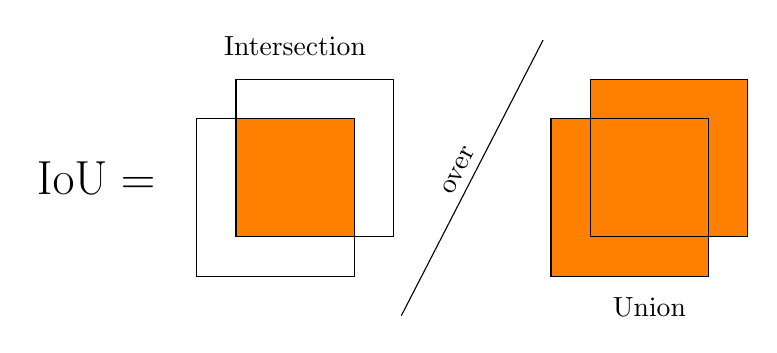
\begin{tikzpicture}
  \node[left] at (-0.4, 1.25) {\LARGE $\mathrm{IoU} = $};
  % Intersection illustration
  \begin{scope}
    \clip (0, 0) rectangle (2, 2);
    \fill[orange] (0.5, 0.5) rectangle (2.5, 2.5);
  \end{scope}
  \draw (0, 0) rectangle (2, 2);
  \draw (0.5, 0.5) rectangle (2.5, 2.5);
  \node[above, yshift=0.5em] at (1.25, 2.5) {Intersection};

  % Division sign
  \draw (2.6, -0.5) -- node[auto, sloped] {over} (4.4, 3);

  % Union illustration
  \begin{scope}[shift={(4.5, 0)}]
    \draw[fill=orange] (0, 0) rectangle (2, 2);
    \draw[fill=orange] (0.5, 0.5) rectangle (2.5, 2.5);
    \draw (0, 0) rectangle (2, 2);
    \node[below, yshift=-0.4em] at (1.25, 0) {Union};
  \end{scope}
\end{tikzpicture}

  \caption{%
    Visualization of single-class IoU metric.
  }%
  \label{fig:iou-metric}
\end{figure}

An alternative metric is the dice coefficient, often called the $F_1$ score as well.
The dice coefficient is defined by dividing twice the area of the intersection by the sum of the areas of the two masks:
%
\begin{equation*}
  \mathrm{F_1}
  =
  \frac{%
    2 \cdot |\mathrm{prediction} \cap \mathrm{truth}|
  }{%
    |\mathrm{prediction}| + |\mathrm{truth}|
  }
  =
  \frac{%
    \mathrm{2 \cdot TP}
  }{%
    2 \cdot \mathrm{TP} + \mathrm{FP} + \mathrm{FN}
  }.
\end{equation*}
%
Again we observe that this metric is bounded to the interval $[0, 1]$, with the same interpretation of the endpoints as with the IoU metric.
The visual representation of this metric is given in~\figref{fig:dice-coefficient}.

\begin{figure}[H]
  \centering
  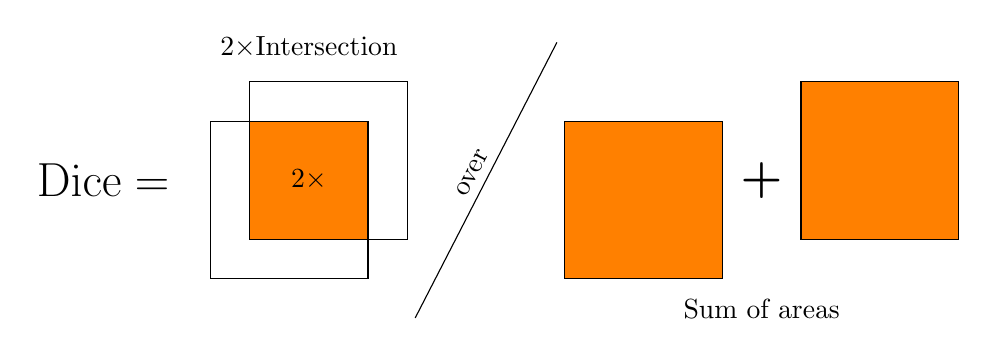
\begin{tikzpicture}
  \node[left] at (-0.4, 1.25) {\LARGE $\mathrm{Dice} = $};

  % Intersection illustration
  \begin{scope}
    \clip (0, 0) rectangle (2, 2);
    \fill[orange] (0.5, 0.5) rectangle (2.5, 2.5);
  \end{scope}
  \draw (0, 0) rectangle (2, 2);
  \draw (0.5, 0.5) rectangle (2.5, 2.5);
  \node[above, yshift=0.5em] at (1.25, 2.5) {$2 \times $Intersection};
  \node at (1.25, 1.25) {$2 \times$};

  % Division sign
  \draw (2.6, -0.5) -- node[auto, sloped] {over} (4.4, 3);

  % Union illustration
  \begin{scope}[shift={(4.5, 0)}]
    \draw[fill=orange] (0, 0) rectangle (2, 2);
    \begin{scope}[shift={(2.5, 0)}]
      \draw[fill=orange] (0.5, 0.5) rectangle (2.5, 2.5);
    \end{scope}
    \draw (0, 0) rectangle (2, 2);
    \node[below, yshift=-0.4em] at (2.5, 0) {Sum of areas};
    \node at (2.5, 1.25) {\LARGE \textbf{+}};
  \end{scope}
\end{tikzpicture}

  \caption{%
    Visualization of the single-class dice coefficient metric, also known as the $F_1$ score.
  }%
  \label{fig:dice-coefficient}
\end{figure}

You may have noticed that these two metrics are quite similar; they involve the same quantities, only weighted differently, and are bounded by to the same domain.
In fact, we can construct an exact relationship between these two metrics\footnote{The following relationship and the ensuing inequality bounds were noted by the \textit{Cross Validated Stack Exchange} user \enquote{Willem} here: \url{https://stats.stackexchange.com/a/276144}.}
%
\begin{equation*}
  \frac{%
    \mathrm{IoU}
  }{%
    \mathrm{F_1}
  }
  =
  \frac{1}{2}
  +
  \frac{%
    \mathrm{IoU}
  }{%
    2
  }.
\end{equation*}
%
The two metrics are therefore always positively correlated, as one metric increases or decreases, the other must necessarily follow suit.
A useful insight for how these two metrics actually differ is to observe how the IoU metric is bounded by the $\mathrm{F_1}$ metric:
%
\begin{equation*}
    \frac{%
      \mathrm{F_1}
    }{%
      2
    }
  \leq
    \mathrm{IoU}
  \leq
    \mathrm{F_1}
\end{equation*}
%
The IoU metric is \textit{always} less than or equal to the $\mathrm{F_1}$ metric, but never less than one half its value.
The fraction $\mathrm{IoU} / \mathrm{F_1}$ is equal to 1 whenever the prediction coincides with the ground truth and is equal to $1/2$ whenever there is no overlap at all.
By drawing an analogy to the $p = 1$ (absolute/Manhattan) norm and $p = 2$ (Euclidean) norm, the $\mathrm{IoU}$ metric is somewhat a reflection of the \textit{worst} performance, while the $\mathrm{F_1}$ metric is more a reflection of the \textit{average} performance of a given prediction.
